\documentclass[journal=jpclcd,manuscript=suppinfo]{achemso}
\pdfoutput=1
\usepackage{gensymb}
\usepackage{amsmath}
\usepackage{graphicx}
\usepackage{epsfig}
\usepackage{multirow}
\usepackage{multicol}

\renewcommand{\thefigure}{S\arabic{figure}}
% Authors / affiliations
% Authors in alphabetical order except for corresponding author (JJF), need 
% to determine if this is the proper order and if we want to have co-first authors!

\author{Jason Codrington$^{\dagger}$}
\affiliation{Department of Chemistry, William Paterson University, 300 Pompton Road, Wayne, NJ, 07470, USA}
\author{Noor Eldabagh$^{\dagger}$}
\affiliation{Department of Chemistry, William Paterson University, 300 Pompton Road, Wayne, NJ, 07470, USA}
\author{Kimberly Fernando$^{\dagger}$}
\affiliation{Department of Chemistry, William Paterson University, 300 Pompton Road, Wayne, NJ, 07470, USA}
\author{Jonathan J. Foley IV}
\affiliation{Department of Chemistry, William Paterson University, 300 Pompton Road, Wayne, NJ, 07470, USA}
\email{foleyj10@wpunj.edu}

%Title of paper
\title{Supporting Information for Unique hot carrier distributions from scattering mediated absorption}
% Date
\date{\today}


% Being document
\begin{document}

\section{Plots of Global Hot-Carrier Distributions}

\begin{figure}
\begin{center}
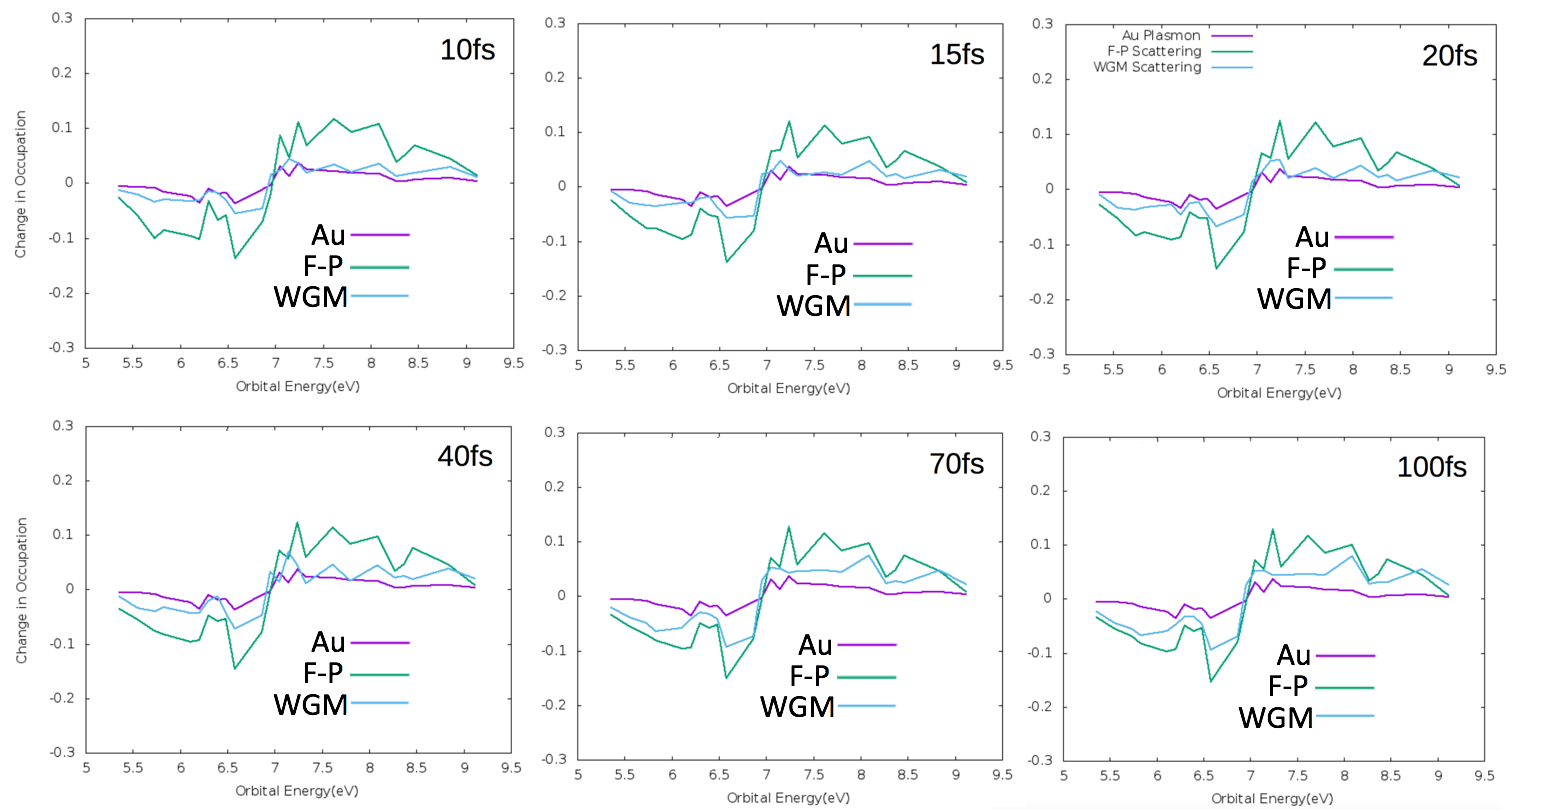
\includegraphics[width=6in]{figs/Au_HotElectronDistribution_Comparison.png}
\caption{Snapshots of changes in occupation of each orbital in the active space of the PIW Au NC model as a measure of instantaneous hot carrier distributions.
The change in orbital occupation is computed from elements of the time-dependent one-electron reduced density matrix ($^1$RDM) relative to
their initial value, $D_p^p(t)-D_P^p(t=0)$ for several timepoints in the simulation.}
\end{center}
\end{figure}


\begin{figure}
\begin{center}
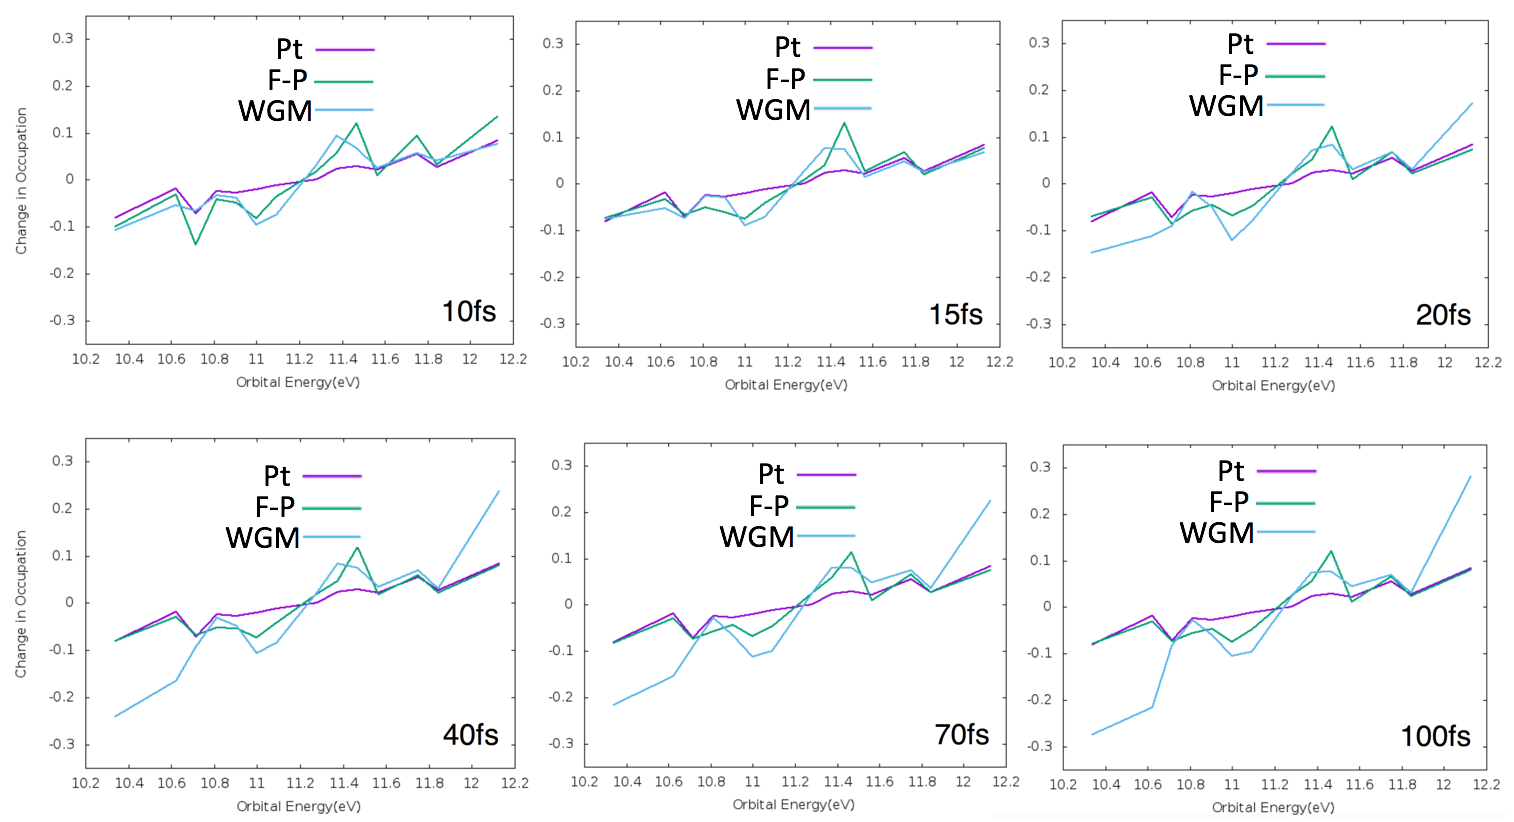
\includegraphics[width=6in]{figs/Pt_HotElectronDistribution_Comparison.png}
\caption{Snapshots of changes in occupation of each orbital in the active space of the PIW Pt NC model as a measure of instantaneous hot carrier distributions.
The change in orbital occupation is computed from elements of the time-dependent one-electron reduced density matrix ($^1$RDM) relative to
their initial value, $D_p^p(t)-D_P^p(t=0)$ for several timepoints in the simulation.  }
\end{center}
\end{figure}



\section{Electronic structure of metal nanocubes}
For cubic metal nanoparticles, we approximate the one-electron orbitals as energy eigenstates of the particle-in-a-cubic-well.  
For a particle confined by a cubic well with length $L$, the potential is 0 when $x<L, y<L, z<L$ and infinity otherwise.  The energy eigenstates
have the form
\begin{equation}
\psi_{nx,ny,nz} = \left(\frac{2}{L}\right)^{3/2} \: {\rm sin}\left(\frac{n_x \: \pi \: x}{L}\right) {\rm sin}\left(\frac{n_y \: \pi \: y}{L}\right) {\rm sin}\left(\frac{n_z \: \pi \: z}{L}\right).
\end{equation}
The energy eigenvalues have the form
\begin{equation}
\epsilon_{nx,ny,nz} = \frac{\hbar^2 \pi^2}{2 \: m \: L^2}\left(n_x^2 + n_y^2 + n_z^2\right).
\end{equation}
The transition dipole operator can be decomposed into its components,
\begin{equation}
{\bf \hat{\mu} } = \hat{\mu}_x \: {\bf i} + \hat{\mu}_y \: {\bf j} + \hat{\mu}_z \: {\bf k}.
\end{equation}
The transition dipole integral components can be evaluated analytically, for example, the 
$x$-component has the form
\begin{align*}
\langle \psi_{nx,ny,nz} |  \hat{\mu}_x | \psi_{nx',ny',nz'} \rangle = e \: \delta_{ny,ny'} \: \delta_{nz,nz'} \:
\frac{L (\pi (n_x - n_x'){\rm sin}(\pi(n_x - n_x'))+{\rm cos}(\pi(n_x-n_x'))-1) }{\pi^2 (n_x - n_x')^2 } \\
-  e \: \delta_{ny,ny'} \: \delta_{nz,nz'} \:
\frac{L (\pi (n_x + n_x'){\rm sin}(\pi(n_x + n_x'))+{\rm cos}(\pi(n_x+n_x'))-1) }{\pi^2 (n_x + n_x')^2 },
\end{align*}
where $\hat{\mu}_x = -e x$.  Analogous expressions can be obtained for expectation values of $\hat{\mu}_y$ and $\hat{\mu}_z$. 

We order the orbitals by a single index $p$ such that $\epsilon_{p+1} \geq \epsilon_p$; that is,
each $\psi_{nx,ny,nz}$ can be uniquely labeled $\psi_p$.
Using the above expressions and following this labeling scheme, the diagonal matrix elements can be evaluated as
\begin{align}
\langle \Phi_0 | \hat{H}(t) | \Phi_0 \rangle &= \sum_{p=1}^{nocc} \epsilon_p \\
\langle \Phi_i^a | \hat{H}(t) | \Phi_i^a \rangle &= \sum_{p=1}^{nocc} \epsilon_p - \epsilon_i + \epsilon_a
\end{align}
and the off-diagonal matrix elements can be evaluated as
\begin{align}
\langle \Phi_0 | \hat{H}(t) | \Phi_i^a \rangle &=  {\bf E}(t) \cdot \langle \psi_i |  {\bf \hat{\mu}} | \psi_a \rangle \\
\langle \Phi_i^a | \hat{H}(t) | \Phi_j^b \rangle &=   {\bf E}(t) \cdot \langle \psi_a |  {\bf \hat{\mu}} | \psi_b \rangle \delta_{ij}  - {\bf E}(t) \cdot \langle \psi_i | {\bf \hat{\mu}} | \psi_j \rangle \delta_{ab}.
\end{align} 



\section{Finite-difference time-domain calculations}
A commercial simulator based on the finite-difference time-domain method~\cite{Lumerical} was used to compute the electric field, $E(t)$
1 \AA $\:$  
away from the nanoparticle surface in each of the scenarios considered.  The displacement
was taken along the $z$-axis, corresponding to the polarization direction of incident light since the strongest
near-field enhancement is expected along this direction.  A grid spacing of 1 \AA $\:$  
in $x$, $y$, and $z$ was utilized
in a cubic region extending 1 nm beyond the metal NP surface, and a non-uniform mesh was utilized otherwise with $dx$, $dy$, $dz \leq 20 nm$.
For each composite structure, a nanoparticle was placed at the surface of the dielectric nanosphere at an angle of
20$^{\circ}$ with respect to the propagation axis of the incident light. In all simulations, light propagates
along the $x$ axis and is polarized along the $z$ axis.  The metal nanoparticles are centered at $y=0$.  
A total-field scattered-field source was used to illuminate the structures.  The FDTD simulations were terminated when the 
ratio of the total energy in the simulation volume to the total energy injected by the illumination source falls below
$10^{-6}$.  Because the WGMs are higher quality factor resonances, longer time is typically required for these simulations
as compared to the plasmonic particles alone.  

The resulting time-domain fields were fed into our TDCIS algorithm, allowing us to simulate the electronic dynamics
driven by rigorously-computed nearfields from scattering and plasmon resonances, which show strong spatiotemporal modification relative
to freely propagating light.  The electric field was scaled by a factor $E_0 \approx 614,000,000 \: V/m$ so that the peak power
of the illumination source is $10^{15} \: W/m^2$.  The electric field was sampled at intervals of approximately 2.8 attoseconds for all simulations, which leads
to a time-step that ensures stability of
the wavefunction propagation with the relevant energy scales of our simulations.  Our TDCIS scheme
requires the evaluation of the electric field at intermediate times between these timesteps, and we use a simple update
based on centered-finite differences to approximate the electric fields at these times.  As an example, if the 
electric field is known at times $t_1$, $t_2 = t_1 + dt$, and $t_3 = t_1 + 2\cdot dt$ where $dt = 2.8 \: as$, and knowledge
of the field is required at some time $t_m = t_2 + m\cdot dt$ where $m$ is non-integer, $E(t_m)$ is estimated as follows: 
\begin{equation}
{\bf E}(t_m) =  {\bf E}(t_2) + \frac{{\bf E}(t_3)-{\bf E}(t_1) }{t_3 - t_1 } \cdot m\cdot dt.
\end{equation}

The optical response of Au and Pt in the FDTD simulations utilizes permittivity data from the work of Johnson and Christy~\cite{JC_PRB_1972} and Palik~\cite{Palik}, respectively.  We assume a static dielectric constant of 2.6 for
the dielectric nanospheres in this work, which is comparable to the visible dielectric constant of titanium dioxide. 

\bibliography{SMHET_SI} 

\end{document}
   

